Due to the non-Abelian nature of the EWK interaction, the associated gauge bosons are allowed to self-interact.
This results in triple and quartic couplings of gauge bosons (TGCs and QGCs, respectively).
The SM allowed TGCs are the $WW\gamma$ and $WWZ$ vertices, which can be measured experimentally via diboson production or through vector boson fusion (VBF).
QGCs predicted by the model include $WWZ\gamma$, $WW\gamma\gamma$, $WWZZ$, and $WWWW$ vertices accessible in triboson production or via vector boson scattering (VBS)\footnote{Vector boson fusion and scattering typically refer to the $s$-channel and $t$-channel exchanges of a vector boson, respectively.  Since both deal with a similar $VV\rightarrow VV$ process, for the remainder of this thesis, \emph{vector boson scattering} will refer to both VBF and VBS.}~\cite{2017.multiboson-at-lhc}.
VBS processes are defined by a $VV\rightarrow VV$ signature, where $V$ represents one of the EWK gauge bosons ($W^{\pm}$, $Z$, or $\gamma$), as shown in Figure~\ref{fig:theory_generic_vbs}.
The actual interaction between the incoming and outgoing vector bosons can be mediated by the exchange of a virtual $V$ or directly via a QGC (as in Figure~\ref{fig:theory_vbs_ewk}), or by the exchange of a Higgs boson (as in Figure~\ref{fig:theory_vbs_higgs}).

\begin{figure}[htbp]
  \centering
  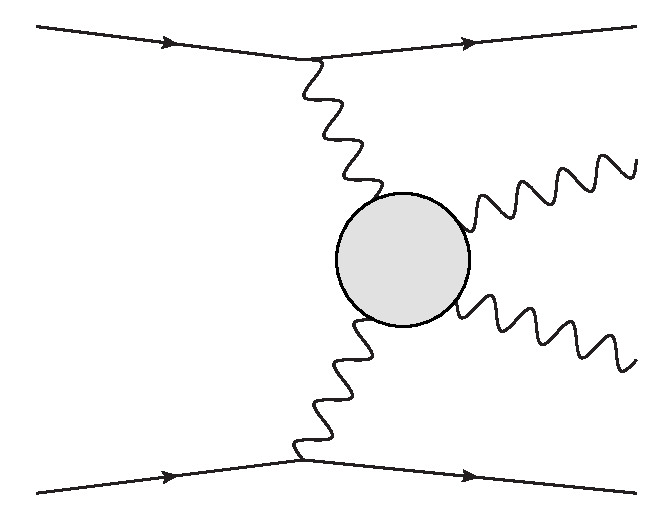
\includegraphics[width=.4\textwidth]{figs/theory/generic_vbs}
  \caption{Feynman diagram of a generic VBS process.  The gray circle represents any interaction with two incoming and two outgoing vector bosons, including any of the diagrams shown in Figures~\ref{fig:theory_vbs_ewk} and \ref{fig:theory_vbs_higgs}.}
  \label{fig:theory_generic_vbs}
\end{figure}

\begin{figure}[htbp]
  \centering
  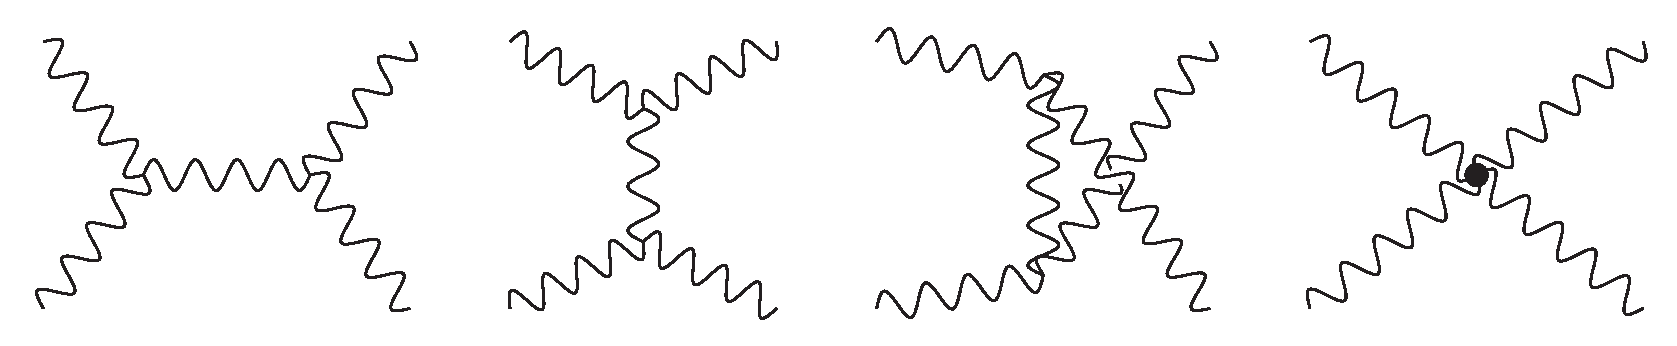
\includegraphics[height=.125\textheight]{figs/theory/vbs_ewk}
  \caption{Leading order $VV\rightarrow VV$ Feynman diagrams involving EWK bosons. From left to right: $s$-channel, $t$-channel, $u$-channel, and the quartic gauge coupling.}
  \label{fig:theory_vbs_ewk}
\end{figure}
\begin{figure}[htbp]
  \centering
  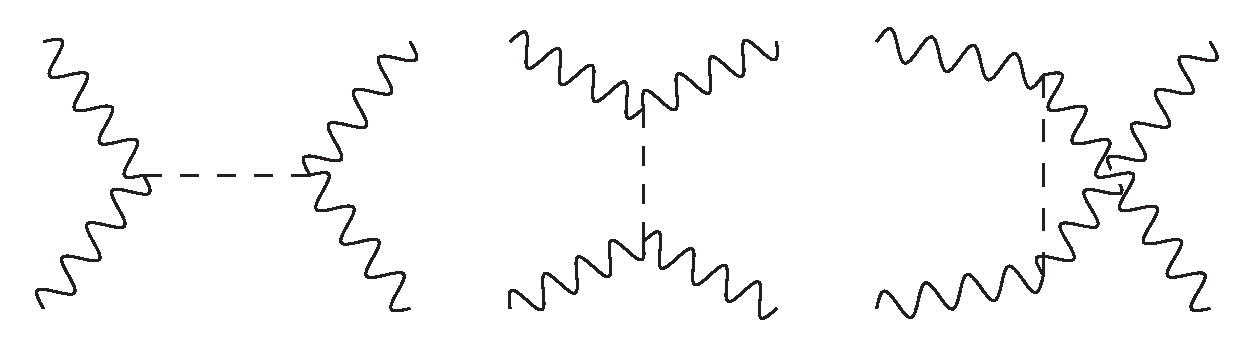
\includegraphics[height=.125\textheight]{figs/theory/vbs_higgs}
  \caption{Leading order $VV\rightarrow VV$ Feynman diagrams involving the exchange of a Higgs boson. From left to right: $s$-channel, $t$-channel, and $u$-channel.}
  \label{fig:theory_vbs_higgs}
\end{figure}

As detailed in the previous section, the Higgs mechanism produces three Goldstone bosons and a Higgs boson.
The Goldstone bosons are then ``eaten'' by the physical gauge bosons, giving them mass and consequently a longitudinal polarization\footnote{A massless spin-1 boson can have one of two transverse polarization states, while a massive spin-1 boson can also be longitudinally polarized.  As a result, only the massive $W^{\pm}$ and $Z$ bosons, and not the massless photon, are sensitive to EWSB.}.
In fact, according to the Electroweak Equivalence Theorem, the high-energy interactions of longitudinal gauge bosons can be accurately described by the Goldstone bosons of the EWSB mechanism~\cite{1997.ewk-equivalence}.
Thus, the scattering of the massive gauge bosons are inextricably linked to EWSB.

It turns out that without a light SM Higgs boson, the scattering amplitude of longitudinally polarized vector bosons grows with center-of-mass energy and ultimately violates unitarity above $\sqrt{s}\approx 1.2\tev$~\cite{1977.ben-lee-weak-interactions, 2009.strong-gauge-boson-scattering}.
Writing down the equations for the transverse and longitudinal polarization vectors for a gauge boson of mass $M_V$~\cite{1990.strong-ww-scattering}:
\begin{equation}
  \epsilon^{\mu}_{\pm} = \frac{1}{\sqrt{2}}(0,0,\pm i, 0)
\end{equation}
\begin{equation}
  \begin{aligned}
    \epsilon^{\mu}_L &= \frac{1}{M_V}(|\vec{p}|, 0, 0, E)\\
                    &= \frac{p^{\mu}}{M_V}+v^{\mu}
  \end{aligned}
  \label{eq:longitudinal_polarization}
\end{equation}
where $v^{\mu}$ is of the order $M_V/E$ and becomes small in the high energy limit, it can be seen that $\epsilon^{\mu}_{L}$ grows with the momentum of the boson $p^{\mu}$.
Therefore, the dominant contribution to the VBS process at high energy comes from the longitudinally polarized gauge bosons~\cite{2012.vbs-thesis-oord}.

% reference diagrams above, then do the matrix element thing (StrongGaugeBosonScatteringTheory.pdf sec 1.1), and cite the figure below
The high-energy behavior of longitudinally polarized vector boson scattering can be explored in the case of opposite-sign $W^{+}W^{-}\rightarrow W^{+}W^{-}$ scattering.
In the high-energy limit ($s >> M_W^2, M_H^2$), the amplitude of $W^{+}W^{-}$ scattering without considering the Higgs contributions (the relevant diagrams in Figure~\ref{fig:theory_vbs_ewk}) can be written as~\cite{2009.strong-gauge-boson-scattering}:
\begin{equation}
  \mathcal{M}_{\textrm{gauge}} = -\frac{g^2}{4M_W^2}u+\mathcal{O}\Bigg(\bigg[\frac{E}{M_W}\bigg]^0\Bigg)
  \label{eq:theory_longitudinal_m_gauge}
\end{equation}
where $g$ is the EWK coupling and $u$ is one of the Mandelstam variables (the others being $s$ and $t$).
The $\mathcal{O}(E^4)$ terms cancel out between the TGC and QGC diagrams~\cite{2012.vbs-thesis-oord}.
What is left is an amplitude proportional to $E^2$ that diverges as $E/M_W\rightarrow\infty$.
However, the amplitude from the diagrams involving the Higgs boson (the relevant diagrams in Figure~\ref{fig:theory_vbs_higgs}) is:
\begin{equation}
  \mathcal{M}_{\textrm{Higgs}} = -\frac{g^2}{4M_W^2}\bigg[\frac{(s-M_W^2)^2}{s-m_H^2}+\frac{(t-M_W^2)^2}{t-M_H^2}\bigg]
\end{equation}
which, in the high-energy limit, reduces to:
\begin{equation}
  \mathcal{M}_{\textrm{Higgs}} = \frac{g^2}{4M_W^2}u+\mathcal{O}\Bigg(\bigg[\frac{E}{M_W}\bigg]^0\Bigg)
  \label{eq:theory_longitudinal_m_higgs}
\end{equation}
Adding the two equations together cancels out the $E^2$ term and leaves only terms constant in energy.
Therefore, with a SM Higgs, the scattering amplitude for longitudinally polarized $W$ bosons no longer diverges.
Plots of the cross section of several $VV\rightarrow VV$ scattering processes are shown in Figure~\ref{fig:theory_vbs_xsec_higgs} with and without a SM Higgs boson.

\begin{figure}[htbp]
  \centering
  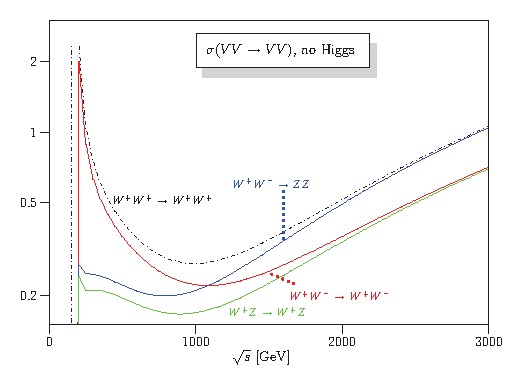
\includegraphics[height=.25\textheight]{figs/ssww_13tev/introduction/vbs_xsec_nohiggs}
  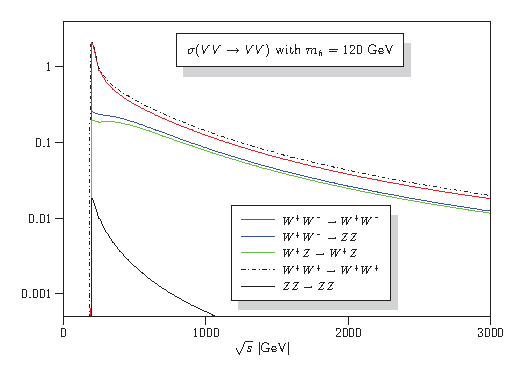
\includegraphics[height=.25\textheight]{figs/ssww_13tev/introduction/vbs_xsec_higgs120}
 
  \caption[Cross sections in nanobarns for five different longitudinally polarized VBS processes as a function of center of mass energy $\sqrt{s}$.  Without a Higgs boson (left), the cross sections grow unbounded with $\sqrt{s}$. With a $120\gev$ Higgs boson (right), the cross sections no longer diverge.]{Cross sections in nanobarns for five different longitudinally polarized VBS processes as a function of center of mass energy $\sqrt{s}$.  Without a Higgs boson (left), the cross sections grow unbounded with $\sqrt{s}$. With a $120\gev$ Higgs boson (right), the cross sections no longer diverge.  Plots taken from~\cite{2008.vbs-resonances-unitarity}.}
  \label{fig:theory_vbs_xsec_higgs}
\end{figure}
